% !TEX root = saveliev_physics_general_course_2.tex
%!TEX TS-program = pdflatex
%!TEX encoding = UTF-8 Unicode


\chapter[THUYẾT VỀ SỰ DẪN ĐIỆN\\ TRONG KIM LOẠI]{THUYẾT VỀ SỰ DẪN ĐIỆN\\ TRONG KIM LOẠI}\label{chap:11}
\chaptermark{THUYẾT VỀ SỰ DẪN ĐIỆN TRONG KIM LOẠI}

\section{Bản chất của hạt mang điện tích trong kim loại}\label{sec:11_1}

Đã có rất nhiều những thí nghiệm được thực hiện nhằm giải mã bản chất của những hạt mang điện tích trong kim loại
Trước hết, chúng ta hãy chú ý vào thí nghiệm được thực hiện bởi nhà vật lý người Đức Carl Riecke (1845-1915).
Ông sử dụng 3 xi lanh---trong đó 2 cái làm từ đồng và cái còn lại làm từ nhôm---đều được mài nhẵn hoàn toàn các đầu.
Sau khi cân, những chiếc xi lanh được đặt theo hàng thẳng theo thứ tự: ống đồng - ống nhôm - ống đồng. 
Một dòng điện được truyền qua dây dẫn tổng hợp này theo một hướng duy nhất trong suốt 1 năm.
Trong suốt thời gian này,một điện tích có giá trị \SI{3.5e6}{\coulomb} đi qua những ống xi lanh .
Việc cân xi lanh đã cho thấy rằng, sự dịch chuyển của dòng điện không làm thay đổi khối lượng của các ống xi lanh.
Khi kiểm tra các đầu ống đã ương tác với nhau bằng kính hiển vị, Không hề có sự liên kết nào từ kim loại này sang kim loại kia được phát hiện.
Kết quả của cuộc thí nghiệm đã chứng mình rằng dòng điện được truyền qua các nguyên tử trong kim loại mà qua các hạt tương tác với nhau ở trong tất cả các loại kim loại.
Hạt electron được tìm ra bởi nhà vật lý Joseph John Thompson vào năm 1897 có thể chính là những hạt Riecke đã giả thuyết.

Để giải thích dòng điện có thể chạy qua kim loại qua các electron tự do, chúng ta cần phải xác định 
Những thí nghiệm đã từng được thực hiện. Nếu kim loại chứa các hạt điện tích dịch chuyển, thì khi một tấm kim loại giảm tốc, các hạt điện tích này sẽ theo tiếp tục di chuyển theo quán tính trong 1 khoảng thời, và kết quả là xung điện sẽ xuất hiện trong tấm.
Giả sử ban đầu có một đoạn dây dẫn di chuyển theo phương của vecto vận tốc $\vec{v}_0$ (\fig{11_1}).
sau đó giảm tốc theo phương của vector gia tốc $\vec{a}$.Vì có quán tính, electron tự do mang điện sẽ tiếp tục di chuyển với gia tốc tương đối $-\vec{a}$ so với dây dẫn
Các hạt mang điện tích được truyền cùng gia tốc trong một dây điện tĩnh nếu một trường điện từ có giá trị $\vec{E}=-m\vec{a}/e'$ được sinh ra bên trong, \ie, Hiệu điện thế giữa hai đầu dây dẫn được tính theo công thức
\begin{equation*}
    \varphi_1 - \varphi_2 = \int_1^2 \vec{E} \ccdot \derivec{l} = -\int_1^2 \frac{m \vec{a}}{e'} \ccdot \derivec{l} = - \frac{mal}{e'},
\end{equation*}

\noindent
($m$ và $e'$ là khối lượng và điện tích của hạt mang điện $l$ là chiều dài của dây dẫn).
Trong trường hợp này, cường độ dòng điện $I = (\varphi_1 - \varphi_2)/R$, trong đó  $R$ là điện trở của dây dẫn ($I$ có dấu dương nếu dòng điện di chuyển cùng phương với dây dẫn).
Do đó, điện tích đi qua mỗi mặt cắt của dây dẫn trong khoảng thời gian $\deriv{t}$ được tính bằng công thức:
\begin{equation*}
    \deriv{q} = I\, \deriv{t} = - \frac{mal}{e'R}\, \deriv{t} = - \frac{ml}{e'R}\, \deriv{v}.
\end{equation*}

\noindent
Lượng điện tích đi qua dây dẫn trong thời gian dây dẫn giảm tốc
\begin{equation}\label{eq:11_1}
    q = \int_1^2 \deriv{q} = - \int_{v_0}^0 \frac{ml}{e'R}\, \deriv{v} = \frac{m}{e'} \frac{lv_0}{R}
\end{equation}

\noindent
(Điện tích được coi có giá trị dương khi hạt mang điện tích di chuyển theo chiều chuyển động của dây dẫn).

\begin{figure}[!htb]
	\begin{center}
		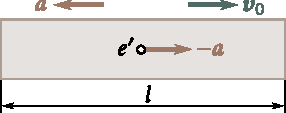
\includegraphics[scale=1]{figures/ch_11/fig_11_1.pdf}
		\caption[]{}
		\label{fig:11_1}
	\end{center}
	\vspace{-0.8cm}
\end{figure}

Vì vậy, bằng việc đo chiều dài $l$, vận tốc ban đầu $v_0$, và điện trở  $R$, và điện tích $q$ khi hạt di chuyển qua dây dẫn đang giảm tốc, chúng ta có thể tìm ra điện tích cơ bản của các hạt mang điện tích, dấu của giá trị phụ thuộc vào hướng của hạt.

Thí nghiệm đầu tiên cho các dây dẫn di chuyển nhanh dần được thực hiện vào năm 1913 bởi hai nhà vật lý học người Xô Viết là Leonid Mandelshtam (1879-1944) và Nikolai Papaleksi (1880-1947).
Họ đã chế một cuộn dây quay quanh trục. Một chiếc điện thoại được kết nối với hai đầu của cuộn dây, và âm thanh được tạo bởi các xung điện đã được nghe qua điện thoại.

Một kết quả được chứng minh bằng toán học đã được thực hiện bởi hai nhà vật lý học người Mý R. Tolman và T. Stewart vào năm 1916. Một ống được làm tự cuộn dây dài \SI{500}{\metre} quay quanh trục với vận tốc quay tuyến tính \SI{300}{\metre\per\second}.
Khi ống dây bị đột ngột bị hãm lại, và hai nhà vật lý đã sử dụng điện kế Ballistic  nhằm đo lượng điện tích đi qua trong mạch dây trong thời gian ống dây bị hãm lại.
Kết quả của tính điện tích cơ bản được tính bởi công thức \eqn{11_1} được cho rằng rất gần với tỉ lệ điện tích trên khối lượng của các hạt electron $e/m$.
Do đó, electron là hạt mang điện đã được chứng minh bằng thực nghiệm.

Dòng điện cỏ thể tạo ra bởi chỉ hiệu điện thế rất rất nhỏ.
Kết quả này đã cho chúng ta nhận xét rằng các hạt mang điện---electron---chuyển động trong kim loại mà gần như không bị cản trở.
Kết quả từ thí nghiệm của Tolman và Stewart cũng cho kết luận tương tự.

Sự tồn tại của electron tự do trong kim loại có thể được giải thích là do trong quá trình các mạng tinh thể được hình thành, các electron hoá trị sẽ tách chúng ra khỏi những nguyên tử trong kim loại
Chúng trở thành ``tập hợp'' thể hiện đặc tính của cả một miếng kim loại.
Nếu một hạt eleectron bị tách ra khỏi , mật độ electron tự do (tưc là số electron $n$ trên một đơn vị thể tích ) tương đương với số nguyên tử trong một đơn vị thể tích.
số hạt electron tự do được cho bởi công thức $(\delta/M)\ab{N}{A}$, trong đó: $\delta$ là mật độ nguyên tử, $M$ là nguyên tử khối, $\ab{N}{A}$ là hằng số Avogrado.
Những giá trị $\delta/M$ của các kim loại dao động trong khoảng \SI{2e4}{\mole\per\metre\cubed} (từ Kali) tới \SI{2e5}{\mole\per\metre\cubed} (tới Beri).
Do đó, chúng ta có những giá trị mật độ electron tự do (hay còn gọi là các electron dẫn):
\begin{equation}\label{eq:11_2}
    n = \text{\SIrange{e28}{e29}{\per\metre\cubed}} \parenthesis{\text{\SIrange{e22}{e23}{\per\centi\metre\cubed}}}.
\end{equation}

\section{Thuyết cơ bản về kim loại}\label{sec:11_2}

Tiếp tục với khái niệm về các electron tự do, Nhà vật lý học người Đức Paul Drude  (1863-1906) đã đưa ra thuyết cơ bản về kim loại, về sau đã được cải tiến bởi H.  Lorentz.
Ông cho rằng các electron dẫn điện trong kim loại có thể coi như các phân tử trong một khí lý tưởng.
Trong khoảng thời gian giữa các lần va chạm, các phân tử chuyển động hoàn toàn tự do, trên  quãng đường tự do trung bình $l$.
Thật vậy, không giống trong một khí các phân tử có quãng đường tự do được xác định dựa vào sự va chạm giữa phân tử này với phân tử khác, các electron không thật sự va chạm với electron khác, mà là do các ion hình thành nên tinh thể kim loại.
Những sự va chạm này gây ra sự cân bằng nhiệt giữa khối khí electron và các tinh thể.

Khi cho rằng kết quả của lý thuyết về khí động lực học có thể áp dụng lên một khối khí electro, chúng ra có thể sử dụng phương trình dưới đểu ước lượng vận tốc trung bình:
\begin{equation}\label{eq:11_3}
    \average{v} = \parenthesis{\frac{8kT}{\pi m}}^{1/2}
\end{equation}

\noindent
[Xem lại phương trình (11.65) ở Vol. I].
Tính toán phương trình này trong nhiệt độ phòng (khoảng \SI{300}{\kelvin}) thì ta có kết quả như dưới đây:
\begin{equation*}
    \average{v} = \parenthesis{\frac{8 \times \num{1.38e-23} \times 300}{ 3.14 \times \num{0.91e-30} }}^{1/2} \approx \SI{e5}{\metre\per\second}.
\end{equation*}

Khi một trường xuất hiện, các chuyển động có trật tự của các electron với tốc độ trung bình  $\average{u}$ bị chồng chất do sự chuyển động hỗn loạn bởi nhiệt xảy ra với vận tốc  $\average{v}$.
Chúng ra dễ dàng tinh toán giá trị của $\average{u}$ bằng phương trình
\begin{equation}\label{eq:11_4}
    j = ne\average{u}
\end{equation}

\noindent
[xem \eqn{5_23}].

 \SI{e7}{\ampere\per\metre\squared} (\SI{10}{\ampere\per\milli\metre\squared}).
Lấy giá trị \SI{e29}{\per\metre\cubed} cho $n$,  ta có
\begin{equation*}
    \average{u} = \frac{j}{en} \approx \frac{\num{e7}}{\num{1.6e-19} \times \num{e29}} \approx \SI{e-3}{\metre\per\second}.
\end{equation*}

\noindent
Do đó, ngay cả khi mật độ điện tích rất cao, tốc độ trung bình của các hạt điện tích có chuyển động theo trật tự  $\average{u}$ có giá trị khoảng $1/\num{e8}$ tốc độ truyền nhiệt trung bình $\average{v}$.
Vì vậy khi tính toán, độ lớn vận tốc tổng hợp $|\vec{v}+\vec{u}|$ có thể được thay thế bằng tốc độ truyền nhiệt $|\vec{v}|$.

Chúng ta tìm ra sự biến thiện giá trị trung bình động năng của electron sinh ra bởi một trường.
Bình phương trung bình của vận tốc là
\begin{equation}\label{eq:11_5}
    \average{(\vec{v}+\vec{u})^2} = \average{\vec{v}^2 + 2\vecdot{v}{u} + \vec{u}^2} = \average{\vec{v^2}} + 2 \average{\vecdot{v}{u}} + \average{\vec{u}^2}.
\end{equation}

\noindent
The two events consisting in that the velocity of thermal motion of the electrons sẽ nhận giá trị $\vec{v}$, trong khi đó vận tốc của hạt chuyển động có trật tự có giá trị  $\vec{u}$, are statistically independent.
Do đó, theo lý thuyết về nhân các xác suất [xem phương trình (11.4) ở Vol. I], ta có $\average{\vecdot{v}{u}} = \average{\vec{v}}\ccdot\average{\vec{u}}$.
Tuy nhiên $\average{\vec{v}}$ có giá trị bằng không, nên số hạng thứ hai trong \eqn{11_5} sẽ biến mất, và nó có dạng
\begin{equation*}
    \average{(\vec{v}+\vec{u})^2} = \average{\vec{v^2}} + \average{\vec{u}^2}.
\end{equation*}

\noindent
Vì thế, động năng của các hạt electron  chuyển động có trật tự tăng theo công thức
\begin{equation}\label{eq:11_6}
    \average{\Delta{\ab{\varepsilon}{k}}} = \frac{m\average{u^2}}{2}.
\end{equation}

\textbf{Định luật Ohm.} Drude cho rằng khi một electron va chạm với ion trong tinh thể, năng lượng sinh ra \eqref{eq:11_6} do hạt electron được chuyển sang ion và tốc độ $u$ as a result of the collision vanishes.
Chúng ta hãy coi rằng sự tăng tốc của trường và của các hạt electron là đồng nhất.
từ đây, dưới sự chuyển động của trường, hạt electron có gia tốc không đổi  $eE/m$,và di chuyển và vận tốc sẽ đạt giá trị
\begin{equation}\label{eq:11_7}
    \ab{u}{max} = \frac{eE}{m} \tau,
\end{equation}

\noindent
trong đó $\tau$ là khoảng thời gian trung bình trôi qua liên tiếp giữa các lần va chạm của hạt electrong với các ion trong mạng tinh thể .

Drude không xét đến sự phân bố các hạt electron với vận tốc và được gán cùng với giá trị của vận tốc $v$ với mọi hạt electron.
Nó gần đúng với
\begin{equation*}
    \tau = \frac{l}{v}
\end{equation*}

\noindent
(chúng tôi nhắc người đọc rằng $|\vec{v}+\vec{u}|$ gần như bằng $|\vec{v}|$).
Sử dụng giá trị $\tau$ ở phương trình \eqn{11_7}, ta có
\begin{equation}\label{eq:11_8}
    \ab{u}{max} = \frac{eEl}{mv}.
\end{equation}

\noindent
Vận tốc $u$ biến thiên tuyến tính trong khoảng thời gian nó đi hết quãng đường  $l$.
Vì vậy, vận tốc trung bình bằng một nửa vận tốc cưc đại:
\begin{equation*}
    \average{u} = \frac{1}{2} \ab{u}{max} = \frac{eEl}{2mv}.
\end{equation*}

\noindent
Đưa phương trình này vào \eqn{11_4}, chúng ta có
\begin{equation*}
    j = \frac{ne^2l}{2mv} E.
\end{equation*}

mật độ dòng điện tỉ lệ thuận với độ mạnh của trường.
Chúng ta đến với định luật Ohm.
Dựa vào phương trình \eqn{5_22}, hệ số tỉ lệ giữa $j$ và $E$ là điện dẫn suất
\begin{equation}\label{eq:11_9}
    \sigma = \frac{ne^2l}{2mv}.
\end{equation}

\noindent
Nếu các electron không va chạm với các ion trong tinh thể, chúng sẽ di chuyển tự do và, khả năng dẫn điện nhiệt của kim loại sẽ lớn vô cùng.
Do đó, \textit{Theo các khái niệm cơ bản, điện trở của kim loại sinh ra do sự va chạm của các electron tư do với các ion trong tinh thể kim loại }.

\textbf{Định luật Joule-Lenz.} cuối quãng đường tự do, một hạt electron tự do sẽ nhận thêm động năng bằng
\begin{equation}\label{eq:11_10}
    \average{\Delta{\ab{\varepsilon}{k}}} = \frac{m \ab{u}{max}^2}{2} = \frac{e^2l^2}{2mv} E^2
\end{equation}

\noindent
[xem \eqns{11_6}{11_8}].
Khi electron va chạm với một ion, theo giả thuyết, nó chuyển hoàn toàn năng lượng nhận được cho tinh thể .
Năng lượng được truyền cho tinh thể  làm tăng nội năng của kim loại hiển nhiên làm kim loại tăng nhiệt.

Every electron experiences on an average $1/\tau=v/l$ collisions a second, communicating each time the energy expressed by \eqn{11_10} to the lattice.
Hence, the following amount of heat should be liberated in unit volume per unit time:
\begin{equation*}
    \ab{Q}{u} = n \frac{1}{\tau} \average{\Delta{\ab{\varepsilon}{k}}} = \frac{ne^2l}{2mv} E^2
\end{equation*}

\noindent
($n$ là số electron truyền trên một đơn vị thể tích).

$\ab{Q}{u}$ là đơn vị thermal power of a current (xem \sect{5_8}).
The factor of $E^2$ coincides with the value given by \eqn{11_9} for $\sigma$.
Passing over in the expression $\sigma E^2$ from $\sigma$ and $E$ to $\rho$ and $j$, chúng ta có được $\ab{Q}{u}=\rho j^2$ biểu diễn định luật Joule-Lenz [xem \eqn{5_39}].

\textbf{Định luật Wiedemann-Franz.} It is known from experiments that in addition to their high electrical conductivity, các kim loại bị chia ra vởi conductivity.
The German physicists G. Wiedemann and R. Franz discovered an empirical law according to which the ratio of the thermal conductivity $\varkappa$ to the electrical conductivity $\sigma$ is about the same for all metals and changes in proportion to the absolute temperature.
Ví dụ, với khôm ở nhiệt độ phòng, tỉ lệ đó bằng \SI{5.8e-6}{\joule\ohm\per\second\per\kelvin}, với đồng là \SI{6.4e-6}{\joule\ohm\per\siemens\per\kelvin}, với chì là \SI{7.0e-6}{\joule\ohm\per\second\per\kelvin}.

Tinh thể phi kim loại cũng có khả năng dẫn nhiệt.
Tuy nhiên, độ dẫn nhiệt của kim loại vượt xa đáng kể so với độ dẫn nhiệt của chất điện môi.
Do đó, theo đó, các electron tự do thay vì mạng tinh thể chịu trách nhiệm truyền nhiệt trong kim loại.
Coi các electron này như một chất khí đơn nguyên tử, chúng ta có thể áp dụng một biểu thức từ lý thuyết động học của chất khí cho tính dẫn nhiệt:
\begin{equation}\label{eq:11_11}
    \varkappa = \frac{1}{3} n m v l c_V
\end{equation}

\noindent
[xem phương trình (16.26) tại Vol. I; mật độ $\rho$ bị thay thế bởi product $nm$, và $\average{v}$ với $v$].
Nhiệt dung đặc trưng của khí đơn nguyên tử là  $c_V = 3R/(2M) = 3k/(2m)$.
sử dụng kết quả từ \eqn{11_11}, ta được
\begin{equation*}
    \varkappa = \frac{1}{2} n k v l.
\end{equation*}

Chia $\varkappa$ trong \eqn{11_9} cho $\sigma$ và thế $3k/(2T)$ với $mv^2/2$, chúng ta có biểu thức
\begin{equation}\label{eq:11_12}
    \frac{\varkappa}{\sigma} = \frac{k m v^2}{e^2} = 3 \parenthesis{\frac{k}{e}}^2 T.
\end{equation}

\noindent
biểu diễn cho định luật Wiedemann-Franz.

Introduction of the numerical values of $k$ và $e$ into \eqn{11_12} yields
\begin{equation*}
    \frac{\varkappa}{\sigma} = \num{2.23e-8}\, T.
\end{equation*}

\noindent
Khi $T = \SI{300}{\kelvin}$, chúng ta được giá trị \SI{3.7e-6}{\joule\ohm\per\second\per\kelvin} cho $\varkappa/\sigma$, điều cũng hợp lý với các dữ liệu từ thí nghiệm (xem các giá trị $\varkappa/\sigma$ trên nhôm, đồng và chì).
It was later established, however, that such a good coincidence is accidental, because when H. Lorentz performed the calculations more accurately, taking
into account the distribution of the electrons by velocities, the value of $2(k/e)^2 T$ was obtained for the ratio $\varkappa/\sigma$, nó không còn đúng với dữ liệu từ các thí nghiệm.

Như vậy, Lý thuyết cơ bản có thể được dùng để giải thích định luật Ohm và định luật Joule-Lenz, cũng như cho một lời giải thích định tính về định luật Wiedemann-Franz.
Song song với đó, nó cùng gặp những trở ngại đáng kể.
They include two basic ones.
Có thể nhận thấy rằng từ phương trình \eqn{11_9} điện trở của kim loại (\ie, the quantity that is the reciprocal of $\sigma$) tỉ lệ thuận với căn bậc hai của $T$.
Thực vậy, chúng ta không có nền tảng nào để thừa nhận các giá trị  $n$ và $l$ phụ thuộc vào nhiệt độ.
Mặt khác, vận tốc chuyển động nhiệt  tỉ lệ thuận với căn bậc hai của  $T$.
Với kết luận lý thuyết này contradicts experimental data according to which the electrical resistance of metals grows in proportion to the first power of $T$, \ie, more rapidly than $T^{1/2}$ [see expression \eqref{eq:5_24}].

Điều trở ngại thứ hai của thuyết cơ bản rằng khối khí electron phải có nhiệt dung mol bằng  $(3/2)R$.
thêm lượng này vào nhiệt dung một kim loại có nhiệt dung $3R$ [xem phương trình (13.1) ở Vol. I], chúng ta có nhiệt dung mol của một kim loại bằng $(9/2)R$ .
Do đó, đúng với thuyết electron cổ điển, nhiệt dung mol phải lớn hơn gấp  $1.5$nhiệt dung mol của các chất điện môi.
Thật ra nhiệt dung riêng của các kim loại không khác đáng kể mấy so với các tinh thể phi kim loại
Chỉ có lý thuyết lượng tử trong kim loại mới có thể giải thích những sự khác biệt này.

\section{Hiệu ứng Hall}\label{sec:11_3}

If a metal plate through which a steady electric current is flowing is placed in a magnetic field perpendicular to it, then a potential difference of $\ab{U}{H} = \varphi_1 - \varphi_2$ (\fig{11_2}) is set up between the plate faces parallel to the directions of the current and field.
This phenomenon was discovered by the American physicist E. Hall in 1879 and is called the \textbf{Hall effect} or the \textbf{galvanomagnetic effect}.

\begin{figure}[!htb]
	\begin{minipage}[t]{0.48\linewidth}
		\begin{center}
			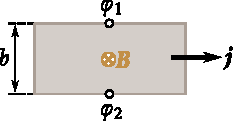
\includegraphics[scale=1]{figures/ch_11/fig_11_2.pdf}
			\caption[]{}
			\label{fig:11_2}
		\end{center}
	\end{minipage}
	\hfill{ }%space{-0.05cm}
	\begin{minipage}[t]{0.48\linewidth}
		\begin{center}
			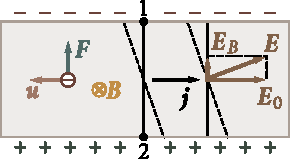
\includegraphics[scale=1]{figures/ch_11/fig_11_3.pdf}
			\caption[]{}
			\label{fig:11_3}
		\end{center}
	\end{minipage}
\vspace{-0.4cm}
\end{figure}

The Hall potential difference is determined by the expression
\begin{equation}\label{eq:11_13}
    \ab{U}{H} = \ab{R}{H} b j B.
\end{equation}

\noindent
Here, $b$ is the width of the plate, $I$ the current density, $B$ the magnetic induction of the field and $ab{R}{H}$ is a constant of proportionality known as the \textbf{Hall coefficient}.

The Hall effect is easily explained by the electron theory.
In the absence of a magnetic field, the current in the plate is due to the electric field $\vec{E}_0$ (\fig{11_3}).
The equipotential surfaces of this field form a system of planes perpendicular to the vector $\vec{E}_0$.
Two of them are shown in the figure by solid straight lines.
The potential at all the points of each surface and, consequently, at points $1$ and $2$ too is the same.
The current carriers---electrons---have a negative charge, therefore, the velocity of their ordered motion $\vec{u}$ is directed oppositely to the current density vector $\vec{j}$.

When the magnetic field is switched on, each carrier experiences the magnetic force $\vec{F}$ directed along side $b$ of the plate and having a magnitude of
\begin{equation}\label{eq:11_14}
    F = euB.
\end{equation}

\noindent
As a result, the electrons acquire a velocity component directed toward the upper (in the figure) face of the plate.
A surplus of negative charges is formed at this face and, accordingly, a surplus of positive charges at the lower face.
Consequently, an additional transverse electric field $\vec{E}_B$ is produced.
When the strength of this field reaches a value such that its action on the charges balances the force given by \eqn{11_14}, a stationary distribution of the charges in a transverse direction will set in.
The corresponding value of $E_B$ is determined by the condition $eE_B = euB$.
Hence,
\begin{equation*}
    E_B = uB.
\end{equation*}

The field $\vec{E}_B$ adds to the field $\vec{E}_0$ to form the resultant field $\vec{E}$.
The equipotential surfaces are perpendicular to the field strength vector.
Consequently, they will turn and occupy the position shown by the dash line in \fig{11_3}.
Points $1$ and $2$ which were formerly on the same equipotential surface now have different potentials.
To find the voltage appearing between these points, the distance $b$ between them must be multiplied by the strength $E_B$:
\begin{equation*}
    \ab{U}{H} = b E_B = b u B.
\end{equation*}

\noindent
Let us express $u$ through $j$, $n$, and $e$ in accordance with the equation $j = neu$.
The result is
\begin{equation}\label{eq:11_15}
    \ab{U}{H} = \frac{1}{ne} b j B.
\end{equation}

\noindent
Equations \eqref{eq:11_13} and \eqref{eq:11_15} coincide if we assume that
\begin{equation}\label{eq:11_16}
    \ab{R}{H} = \frac{1}{ne}.
\end{equation}

Inspection of \eqn{11_16} shows that by measuring the Hall coefficient, we can find the concentration of the current carriers in a given metal (\ie, the number of carriers per unit volume).

An important characteristic of a substance is the mobility of the current carriers in it.
By the mobility of the current carriers is meant the average velocity acquired by the carriers at unit electric field strength.
If the carriers acquire the velocity $u$ in a field of strength $E$, then their mobility $u_0$ is
\begin{equation}\label{eq:11_17}
    u_0 = \frac{u}{E}.
\end{equation}

\noindent
The mobility can be related to the conductivity $\sigma$ and to the carrier concentration $n$.
For this purpose, let us divide the equation $j=neu$ by the field strength $E$.
Taking into account that $j/E=\sigma$ and $u/E=u_0$, we get
\begin{equation}\label{eq:11_18}
    \sigma = ne u_0.
\end{equation}

Having measured the Hall coefficient $\ab{R}{H}$ and the conductivity $\sigma$, we can use \eqns{11_16}{11_18} to find the concentration and
mobility of the current carriers in the relevant specimen.

The Hall effect is observed not only in metals, but also in semiconductors.
The sign of the effect can be used to see whether a semiconductor belongs to the n- or p-type\footnote{In n-type semiconductors, the current carriers are negative, and in p-type ones they are positive (see Vol. III).}.
Figure \ref{fig:11_4} compares the Hall effect for specimens with positive and negative carriers.
The direction of the magnetic force is reversed both when the direction of motion of the charge changes and when its sign is reversed.
Hence, when the current and field have the same direction, the magnetic force exerted on positive and negative carriers has the same direction.
Therefore, with positive carriers, the potential of the upper (in the figure) face is higher than that of the lower one, and with negative carriers the potential is lower.
We can thus establish the sign of the current carriers after determining that of the Hall potential difference.

\begin{figure}[!htb]
	\begin{center}
		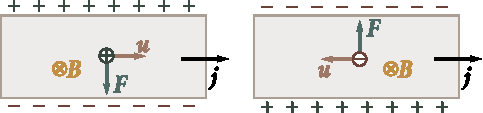
\includegraphics[scale=1]{figures/ch_11/fig_11_4.pdf}
		\caption[]{}
		\label{fig:11_4}
	\end{center}
	\vspace{-0.8cm}
\end{figure}

It is of interest to note that in some metals the sign of $\ab{U}{H}$ corresponds to positive current carriers.
This anomaly is explained by the quantum theory.
